\section{Лекция 13.02.2020}

\subsection{Симметризация билинейной формы и поляризация квадратичной формы}

\begin{comment}~
    \begin{enumerate}
        \item Билинейная форма $\sigma(x, y) = \frac{1}{2} \left(\beta(x, y) + \beta(y, x)\right)$ называется \textit{симметризацией} билинейной формы $\beta$.

            Если $B$ и $S$ --- матрицы билинейных форм $\beta$ и $\sigma$ в некотором базисе, то $S = \frac{1}{2} (B + B^{T})$.

        \item Симметричная билинейная форма $\beta(x, y) = \frac{1}{2} \left[Q(x + y) - Q(x) - Q(y)\right]$ называется \textit{поляризацией} квадратичной формы $Q$.
    \end{enumerate}
\end{comment}

\begin{definition}
    Матрицей квадратной формы $Q$ в базисе $\E$ называется матрица соответствующей симметричной билинейной формы (поляризации) в базисе $\E$.

    Обозначение: $B(Q, \E)$.
\end{definition}

\begin{example}
    Пусть $Q(x_1, x_2) = x_1^2 + x_1 x_2 + x_2^2$.

    Если $\E$ --- стандартный базис, то $B(Q, \E) = \begin{pmatrix} 1 & \frac{1}{2} \\ \frac{1}{2} & 1 \end{pmatrix}$.
\end{example}


\subsection{Канонический вид квадратичной формы}

\begin{definition}
    Квадратичная форма $Q$ имеет в базисе $\E$ \textit{канонический вид}, если $B(Q, \E)$ диагональна.

    Если $B(Q, \E) = \diag(b_1, b_2, \dots, b_n)$, то $Q(x_1, \dots, x_n) = b_1 x_1^2 + b_2 x_2^2 + \dots + b_n x_n^2$.
\end{definition}


\subsection{Теорема о приведении квадратичной формы к каноническому виду. Метод Лагранжа}

\begin{theorem}
    Всякую квадратичную форму путём замены базиса можно привести к каноническому виду.
\end{theorem}

\begin{proof}[Доказательство (метод Лагранжа)]
    Индукция по $n$:
    \begin{description}
    \item[База] $n = 1 \implies Q(x) = b x_1^2$ --- канонический вид.
    \item[Шаг] Пусть утверждение доказано для $< n$, докажем для $n$.

        Пусть $B = B(Q, \E)$ --- матрица квадратичной формы в исходном базисе $\E$.
        \begin{equation*}
            Q(x) = \sum_{i = 1}^{n} b_{ii} x_i^2 + \sum_{1 \leq i < j \leq n}^{n} 2 b_{ij} x_i x_j
        .\end{equation*}

        \begin{enumerate}[start=0,label=Случай \arabic*.]
        \item
            $b_{ij} = 0 \ \forall i, j$ --- доказывать нечего.
        \item
            $\exists i : b_{ii} \neq 0$. Сделав перенумерацию, считаем $b_{11} \neq 0$.

            Тогда,
            \begin{align*}
                Q(x_1, \dots, x_n)
                &= b_{11} x_1^2 + 2b_{12} x_1 x_2 + \dots + 2 b_{1n} x_1 x_n + Q_1(x_2, \dots, x_n) \\
                &= b_{11} \left(x_1^2 + 2\frac{b_{12}}{b_{11}} x_1 x_2 + \dots + 2\frac{b_{1n}}{b_{11}} x_1 x_n\right) + Q_1(x_2, \dots, x_n) \\
                &= b_{11} \Bigg(\underbrace{x_1 + \frac{b_{12}}{b_{11}} x_2 + \dots + \frac{b_{1n}}{b_{11}} x_n}_{x'_1}\Bigg)^2 \underbrace{ - b_{11} \left(\frac{b_{12}}{b_{11}}x_2 + \dots + \frac{b_{1n}}{b_{11}} x_n\right)^2 + Q_1(x_2, \dots, x_n)}_{Q_2(x_2, \dots, x_n)} \\
                &= b_{11} (x_1')^2 + Q_2 (x'_2, \dots, x'_n)
            ,\end{align*}
            где
            \begin{equation*}
                \begin{cases}
                    x'_1 &= x_1 + \frac{b_{12}}{b_{11}} x_2 + \dots + \frac{b_{1n}}{b_{11}} x_n, \\
                    x'_2 &= x_2, \\
                         &\vdots \\
                    x'_n &= x_n.
                \end{cases}
            \end{equation*}

            Здесь важно проследить, что замена действительно соответствует замене базисов (то есть является невырожденной).

            Вспомним как происходит замена базиса:

            \begin{equation*}
                \boxed{
                    \begin{aligned}
                        \E' &= \E \cdot C \\
                        \begin{pmatrix} x_1 \\ \dots \\ x_n \end{pmatrix} &= C \cdot \begin{pmatrix} x'_1 \\ \dots \\ x'_n \end{pmatrix}
                    \end{aligned}
                }
            \end{equation*}

            Выразим $x$ через $x'$ и запишем матрицу перехода:
            \begin{equation*}
                \begin{cases}
                    x_1 &= x'_1 - \frac{b_{12}}{b_{11}} x'_2 - \dots - \frac{b_{1n}}{b_{11}} x'_n, \\
                    x_2 &= x'_2, \\
                        &\vdots \\
                    x_n &= x'_n.
                \end{cases}
                \hspace{3cm}
                C = \begin{pmatrix} 
                    1 & - \frac{b_{12}}{b_{11}} & \dots & -\frac{b_{1n}}{b_{11}} \\
                    0 & 1 & \dots & 0 \\
                    \vdots & \vdots & \ddots & \vdots \\
                    0 & 0 & \dots & 1
                \end{pmatrix}
            \end{equation*}

            По предположению индукции, $Q_2$ можно привести к каноническому виду.

        \item
            $b_{ii} = 0 \ \forall i$, но $\exists i, j, i \neq j$, такие что $b_{ij} \neq 0$.

            Выполнив перенумерацию считаем, что $b_{12} \neq 0$.

            Сделаем замену и выпишем матрицу перехода:
            \begin{equation*}
                \begin{cases}
                    x_1 &= x'_1 + x'_2, \\
                    x_2 &= x'_1 - x'_2, \\
                    x_3 &= x'_3, \\
                        &\vdots \\
                    x_n &= x'_n.
                \end{cases}
                \hspace{3cm}
                C = \begin{pmatrix} 
                    1 & 1 & 0 & \dots & 0 \\
                    1 & -1 & 0 & \dots & 0 \\
                    0 & 0 & 1 & \dots & 0 \\
                    \vdots & \vdots & \vdots & \ddots & \vdots \\
                    0 & 0 & 0 & \dots & 1
                \end{pmatrix}
            \end{equation*}

            Получаем $Q(x) = b_{12} x_1^2 - b_{12} x_2^2 + \underbrace{\dots\dots\dots\dots}_{\text{нет квадратов}}$, мы попали в случай 1.
            \qedhere
        \end{enumerate}
    \end{description}
\end{proof}

\begin{comment}
    Базис, в котором $Q$ имеет канонический вид, а так же сам этот вид, определены, вообще говоря, неоднозначно.
\end{comment}

\begin{example}
    $Q(x_1, x_2) = x_1^2 + x_2^2$.

    Замена $\E' = (2e_1, 2e_2) \ \left[x_1 = 2'x_1, x_2 = x'_2\right]$,

    Тогда, $Q(x'_1, x'_2) = 4x'^2_1 + 4x'^2_2$.
\end{example}


\subsection{Угловые миноры матрицы квадратичной формы}

Пусть $\E = (e_1, \dots, e_n)$ --- базис пространства $V$.

Рассмотрим систему векторов $e'_1, \dots, e'_n$ следующего вида:

$e'_1 = e_1$,

$e'_2 \in e_2 + \left< e_1 \right>$,

$e'_3 \in e_3 + \left< e_1, e_2 \right>$,

$\dots$

$e'_n \in e_n + \left< e_1, \dots, e_{n - 1} \right>$.

Для любого $k = 1 \dots n$ имеем $(e'_1, \dots, e'_k) = (e_1, \dots, e_k) \cdot C_k$, где
\begin{equation*}
    C_k = \begin{pmatrix} 
        1 & \star & \dots & \star & \star \\
        0 & 1 & \ddots & \star & \star \\
        \vdots & \vdots & \ddots & \ddots & \vdots \\
        0 & 0 & \dots & 1 & \star \\
        0 & 0 & \dots & 0 & 1
    \end{pmatrix} \in M_k(F)
.\end{equation*}

Так как $\det C = 1 \neq 0$, то $e'_1, \dots, e'_k$ линейно независимы и $\left< e_1, \dots, e_k \right> = \left< e'_1, \dots, e'_k \right>$.

В частности, $e'_1, \dots, e'_n$ --- базис $V$.

Заметим, что $C_k$ --- левый верхний $k \times k$ блок в $C_n$.

Пусть $Q \colon V \to F$ --- квадратичная форма, $\beta$ --- соответствующая симметричная билинейная форма.

$B := B(Q, \E)$.

$B_k$ --- левый верхний $k \times k$ блок в $B$.

$\delta_k := \delta_k(Q, \E) := \det B_k(Q, \E)$ --- $k$-й угловой минор матрицы $B$.

Для удобства, $\delta_0 := 1$.

\begin{lemma}
    Пусть $(e'_1, \dots, e'_n) = \E'$ --- базис $V$ описанного выше вида и $\delta'_k = \delta_k(Q, \E')$. Тогда, $\delta'_k = \delta_k \ \forall k$.
\end{lemma}

\begin{proof}
    Пусть $B' = B(Q, \E')$ и $B'_k = B_k(Q, \E')$.

    Так как $\left< e'_1, \dots, e'_k \right> = \left< e_1, \dots, e_k \right>$, то $B'_k = C_k^T B_k C_k$.
    Отсюда, $\delta'_k = \det B'_k = \underbrace{\det C_k^T}_1 \det B_k \underbrace{\det C_k}_1 = \det B_k = \delta_k$.
\end{proof}


\subsection{Метод Якоби приведения квадратичной формы к каноническому виду}


\begin{theorem}
    Пусть $\delta_k \neq 0 \ \forall k = 1, \dots, n$.

    Тогда, $\exists!$ базис $\E' = (e'_1, \dots, e'_n)$ в $V$, такой что
    \begin{enumerate}
    \item $\E'$ имеет описанный выше вид;
    \item В базисе $\E'$ $Q$ принимает канонический вид

        $Q(x'_1, \dots, x'_n) = \delta_1 x'^2_1 + \frac{\delta_2}{\delta_1} x'^2_2 + \dots + \frac{\delta_n}{\delta_{n - 1}} x'^2_n$.

        То есть $B(Q, \E') = \diag\left(\delta_1, \frac{\delta_2}{\delta_1}, \dots, \frac{\delta_n}{\delta_{n - 1}}\right)$
    \end{enumerate}
\end{theorem}

\begin{proof}
    Индукция по $n$.

    \begin{description}
    \item[База] $n = 1 \implies $ верно.
    \item[Шаг] Пусть доказано для $< n$, докажем для $n$.

        Применяя предположение индукции к ограничению квадратичной формы на подпространство $\left< e_1, .., e_{n - 1} \right>$ получаем, что $\exists$ требуемый базис $e'_1, \dots, e'_{n - 1}$ в $\left< e_1, \dots, e_{n - 1} \right>$ нужного вида.

        Тогда, $B(Q, (e'_1, \dots, e'_{n - 1}, e_n))$ имеет вид 
        \begin{equation*}
            \left(\begin{array}{cccc|c}
                \delta_1 & 0 & \dots & 0 & \star \\
                0 & \frac{\delta_2}{\delta_1} & \dots & 0 & \star \\
                \vdots & \vdots & \ddots & \vdots & \vdots \\
                0 & 0 & \dots & \frac{\delta_{n - 1}}{\delta_{n - 2}} & \star \\
                \hline
                \star & \star & \dots & \star & \star
            \end{array}\right)
        .\end{equation*}

        Ищем $e'_n$ в виде
        \begin{equation*}
            e'_n = e_n + \lambda_1 e'_1 + \dots + \lambda_{n - 1} e'_{n - 1}
        .\end{equation*}

        Для любого $k = 1, \dots, n - 1$
        \begin{align*}
            \beta(e'_n, e'_k) &= \beta(e_n + \lambda_1 e'_1 + \dots + \lambda_{n - 1} e'_{n - 1}, e'_k) \\
            &= \beta(e_n, e'_k) + \lambda_1 \beta(e'_1, e'_k) + \dots + \lambda_{n - 1} \beta(e'_{n - 1}, e'_k) \\
            &= \beta(e_n, e'_k) + \lambda_k \beta(e'_k, e'_k) \\
            &= \beta(e_n, e'_k) + \lambda_k \frac{\delta_k}{\delta_{k - 1}}
        .\end{align*}

        Хотим, $\beta(e'_n, e'_k) = 0 \ \forall k = 1, \dots, n - 1 \iff \lambda_k = -\beta(e_n, e'_k) \frac{\delta_{k - 1}}{\delta_k}$.

        Тогда в базисе $\E' = (e'_1, \dots, e'_n)$ матрица $Q$ равна
        \begin{equation*}
            \begin{pmatrix} 
                \delta_1 & 0 & \dots & 0 & 0 \\
                0 & \frac{\delta_2}{\delta_1} & \dots & 0 & 0 \\
                \vdots & \vdots & \ddots & \vdots & \vdots \\
                0 & 0 & \dots & \frac{\delta_{n - 1}}{\delta_{n - 2}} & 0 \\
                0 & 0 & \dots & 0 & ?
            \end{pmatrix}
        .\end{equation*}

        По лемме, $\delta_n = \delta'_n = \delta_1 \cdot \frac{\delta_2}{\delta_1} \cdot \dots \cdot \frac{\delta_{n - 1}}{\delta_{n - 2}} \cdot ? = \delta_{n - 1} \cdot ? \implies ? = \frac{\delta_n}{\delta_{n - 1}}$.

        Единственность следует из явной формулы для $\lambda_k$.
        \qedhere
    \end{description}
\end{proof}

\begin{center}
    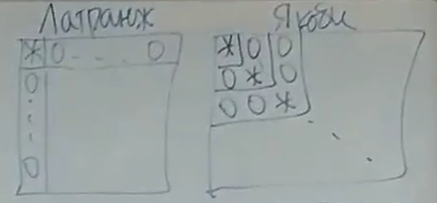
\includegraphics[height=5cm]{lecture20_matrix}
\end{center}


\subsection{Нормальный вид квадратичной формы над полем $\RR$}

\begin{definition}
    Квадратичная форма над $\RR$ имеет \textit{нормальный вид} в базисе $\E$, если в этом базисе
    \begin{equation*}
        Q(x_1, \dots, x_n) = \epsilon_1 x_1^2 + \dots + \epsilon_n x_n^2
    ,\end{equation*}
    где $\epsilon_i \in \{-1, 0, 1\}$.
\end{definition}


\subsection{Приведение квадратичной формы над R к нормальному виду}

\begin{corollary}[из метода Лагранжа]
    Для всякой квадратичной формы $Q$ над $\RR$ существует базис, в котором $Q$ имеет нормальный вид.
\end{corollary}

\begin{proof}
    Из теоремы знаем, что существует базис $\E$, в котором $Q$ имеет канонический вид
    \begin{equation*}
        Q(x_1, \dots, x_n) = b_1 x_1^2 + \dots + b_n x_n^2
    .\end{equation*}

    Делаем замену
    \begin{equation*}
        x_i = \begin{cases}
            \frac{x'_i}{\sqrt{|b_i|}}, &b_i \neq 0 \\
            x_i, &b_i = 0
        \end{cases}
    .\end{equation*}

    Тогда в новых координатах $Q(x'_1, \dots, x'_n) = \epsilon_1 x'^2_1 + \dots + \epsilon_n x'^2_n$,

    \begin{equation*}
        \epsilon_i = \sgn b_i = \begin{cases}
            1, &b_i > 0 \\
            0, &b_i = 0 \\
            -1, &b_i < 0
        \end{cases}
    .\end{equation*}
\end{proof}
